\section{Interpolación}
El problema de aproximación de funciones a través de técnicas de interpolación aparece de manera recurrente en diferentes aplicaciones de ingeniería. Por ejemplo en el ajuste de datos de laboratorio cuando estos son relativamente estables, en la visualización de funciones y en el desarrollo de métodos de solución de problemas de valores en la frontera. La teoría de interpolación es de especial interés en el método de los elementos finitos, en el cual se obtienen valores de los desplazamientos en una serie de puntos y estos se usan, conjuntamente con métodos de interpolación para determinar deformaciones y tensiones. En esta sección se estudiarán los aspectos fundamentales del problema de interpolación de funciones a partir de polinomios de Lagrange. 
\subsection{Planteamiento del problema}

Sea $f(x)$ una función desconocida analiticamente pero con valores conocidos de manera discreta en $n$ puntos $x_1,  x_2, \cdots, x_n$. Queremos conocer (o interpolar) el valor de $f(x)$ en un punto arbitrario  $x \in [x_1, x_n]$ y que es diferente a uno de los $n-$puntos.

El problema de interpolación consiste precisamente en determinar el valor desconocido de $f(x)$ usando los valores conocidos $\left\{f_1,f_2,...,f_n\right\}$. Por ejemplo, tomemos los valores discretos de una función $f(x)$ que se tiene en la \cref{tab:interp_puntos} y que se muestran mediante circulos negros en la \cref{fig:interp_puntos}.

\begin{center}
	\begin{tabular}{rr}
		\hline
		$x$ & $f(x)$ \\
		\hline 
		$-1.0$  & $-7.000$  \\
		$-0.5$  & $-9.125$  \\
		$ 0.00$  & $-10.00$  \\
		$ 0.50$  & $-8.875$  \\
		$ 1.00$  & $-5.000$  \\
		\hline
	\end{tabular}
	\captionof{table}{Valores conocidos de la función $f(x)$.}
	\label{tab:interp_puntos}
\end{center}
%
\begin{figure}[H]
	\centering
	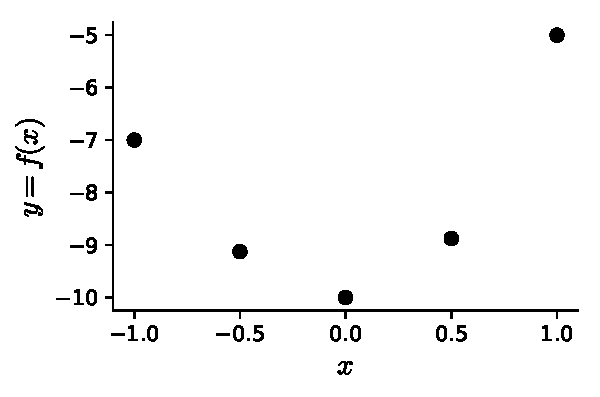
\includegraphics[height=2.5 in]{interp_puntos.pdf}
	\caption{Puntos correspondientes a valores conocidos de una función. Se desea determinar el valor de la función para puntos diferentes a los de medición.}
	\label{fig:interp_puntos}
\end{figure}


Para determinar los valores desconocidos de la función $f(x)$ usando los valores dados $\left\{f_1,f_2,...,f_n\right\}$ el problema se resuelve en dos pasos:

\begin{enumerate}
	\item  Se propone una función de interpolación que pase por los $n$ valores conocidos. Este paso se ilustra mediante la línea punteada de la \cref{fig:interp_continua}. En nuestro caso, propondremos funciones polinomiales.
		
	\item Una vez se disponga de la función de interpolación esta puede ser usada para predecir el valor en puntos arbitrarios. Si se dispone de $n$ datos o valores conocidos de la función es posible proponer un polinomio de interpolación de orden $n-1$. Sin embargo, si se dispone de un número alto de valores conocidos de la función, puede resultar contraproducente el realizar la aproximación usando un polinomio de alto orden.
	
	
		\begin{figure}[H]
		\centering
		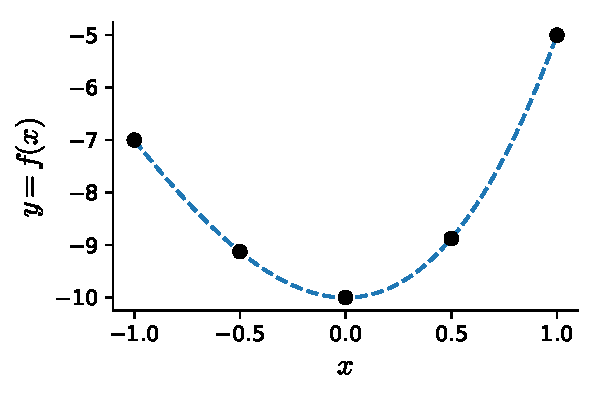
\includegraphics[height=2.5 in]{interp_continua.pdf}
		\caption{Polinomio de interpolación usando los $n$-datos. El polinomio resultante es de orden $n-1$.}
		\label{fig:interp_continua}
	\end{figure}
	
	Alternativamente, es posible dividir el dominio del problema en sub-dominios y proceder con interpolaciones locales. Esta alternativa se muestra en la \cref{fig:interp_tramos} en la cual se realiza una interpolación lineal entre pares de puntos.
	\begin{figure}[h]
		\centering
		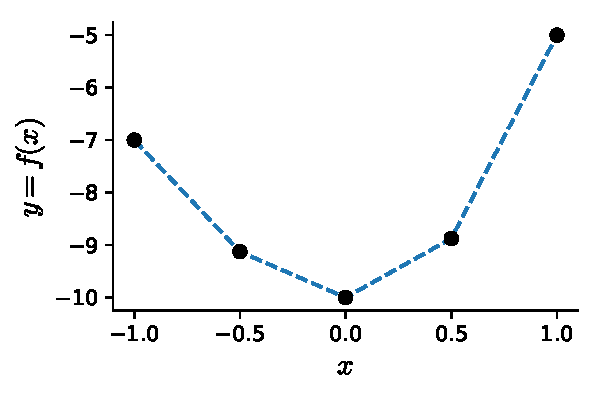
\includegraphics[height=2.5 in]{interp_tramos.pdf}
		\caption{Función de interpolación  definida por tramos usando pares de puntos para producir polinomios locales de orden $1$.}
		\label{fig:interp_tramos}
	\end{figure}
	
\end{enumerate}

\paragraph*{Ejemplo: Una aplicación en ingeniería civil.}
En este ejemplo se presenta a manera de pregunta un problema típico de interpolación en Ingeniería Civil. En este caso la interpolación requerida es para una fución en el plano. Como veremos de manera formal mas adelante, la solución de este tipo de problemas usa como ingrediente fundamental la solución al problema de interpolación de funciones uni-dimensionales.

La \cref{fig:ram} muestra la distribución de los equipos de registro sísmico que conforman la red acelerográfica de Medellín. Tras la ocurrencia de un evento sísmico cada uno de estos equipos registra el movimiento del terreno en el sitio particular. Dichos movimientos son usados posteriormente para calcular espectros de respuesta para uso en análisis y diseño de estructuras sismo-resistentes.

\begin{figure}[H]
\centering
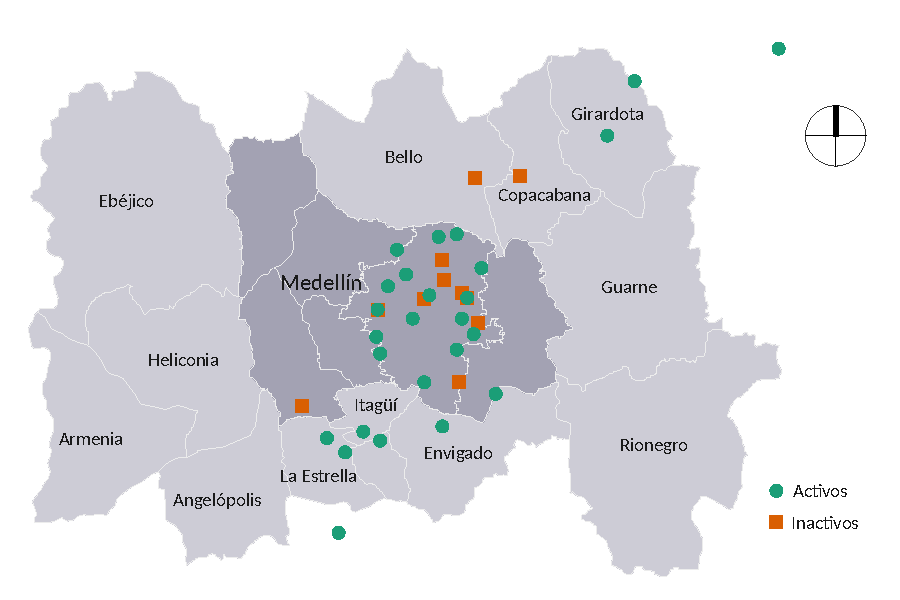
\includegraphics[width=10cm]{red_acelerografica.pdf}
\caption{Red acelerográfica de Medellín. Los círculos verdes representan estaciones activas. Mientras que los cuadrados naranja son estaciones inactivas. Datos de julio de 2017, tomados de SIATA\cite{SIATA_acelerografica}}
\label{fig:ram}
\end{figure}

Como se aprecia en la figura, la cobertura espacial es limitada, lo que dificulta el problema de análisis estructural en zonas de la ciudad donde no se disponga de instrumentación. Se requiere entonces usar una alternativa numérica que permita determinar los espectros de respuesta en sitios carentes de instrumentación de manera consistente con los resultados instrumentales. En términos matemáticos el problema corresponde a uno de interpolación o cálculo de valores de una función en un punto arbitrario usando valores conocidos de la función en un número limitado de puntos. En esta sección se estudiarán los aspectos teóricos fundamentales para resolver problemas de interpolación sobre dominios unidimensionales (1D) y bidimensionales (2D). Inicialmente se estudiará el método clásico de interpolación a partir de los polinomios de Lagrange y posteriormente, se discutirá la generalización de este esquema a dominios 2D (como en el problema de la red 
acelerográfica de Medellín). Posteriormente se discutirán algunas patologías o inconvenientes numéricos propios del problema.

\subsection{Teorema de interpolación de Lagrange}
Dado un conjunto de $n$-puntos $\{ (x_1, y_1),\cdots,(x_n, y_n)\}$, donde $y_n 
\equiv f({x_n})$ entonces: existe un único polinomio $p(x)$ de orden a lo sumo 
$(n-1)$ tal que $p(x_i) = f(x_i)$ para $i = 1, 2, \cdots, n$.

El polinomio está dado por

\begin{equation}\label{eq:interp_pol}
  p(x) = L_1(x) f(x_1)+L_2(x) f(x_2)+...+L_n(x) f(x_n)\, ,
\end{equation}

para $i = 1, 2, \cdots, n$ donde

\begin{equation}\label{eq:interp_coef}
  L_i(x) = \prod_{\substack{j = 1\\ i \ne j}}^n \frac{(x - x_j)}{(x_i - x_j)}\, 
  ,
\end{equation}

y donde se debe notar que

\[L_i(x_j) =
\begin{cases}
1,\quad \text{si } i = j\\
0,\quad \text{si } i \neq j\, .
\end{cases}\]

\begin{tcolorbox}
En el lenguaje matemático es común denominar la función $p(x)$ con la que 
se aproxima la función $f(x)$ como \textbf{polinomio de interpolación} 
mientras que cada uno de los polinomios de Lagrange del tipo $L_i(x)$ se 
denominan \textbf{polinomios interpolantes} aunque también es posible 
encontrarlos como polinomios de interpolación. Será fácil reconocer quien 
es quien de acuerdo al contexto. De otro lado, en el lenguaje del método de 
los elementos finitos donde es frecuente el uso de técnicas de 
interpolación es común denominar a los polinomios interpolantes como 
funciones de forma o funciones base y a los puntos donde la función es 
conocida como nodos.
\end{tcolorbox}


\paragraph{Ejemplo: Interpolación de una fución usando 3 valores conocidos.}
El \cref{tab:interp_tres} contiene los valores exactos de la función $f(x) = {x^3} + 4{x^2} - 10$ en los puntos $x^1 =  - 1.0$, $x^2 =  + 1.0$ y $x^3 = 0.0$. Usando polinomios de interpolación de Lagrange proponer una función de interpolación que permita conocer el valor de la función y su primera derivada en $x=0.7$.
\begin{center}
\begin{tabular}{ll}
  \hline
  $x$ & $f(x)$ \\
  \hline 
  $-1.0$  & $-7.000$  \\
  $ 0.00$  & $-10.00$  \\
  $ 1.00$  & $-5.000$  \\
  \hline
\end{tabular}
\captionof{table}{Valores conocidos de la función $f(x) = {x^3} + 4{x^2} - 10$.}
\label{tab:interp_tres}
\end{center}

Inicialmente determinemos los polinomios interpolantes correspondientes a 
los puntos $x_1 = -1.0$, $x_2 =  1.0$ y $x_3 = 0.0$. Usando la 
\cref{eq:interp_coef}, obtenemos

\begin{align*}
& L_1(x) = \frac{(x - x_2)(x - x_3)}{(x_1 - x_2)(x_1 - x_3)} = -\frac{1}{2}(1 
- x)x\\
& L_2(x) = \frac{(x - x_1)(x - x_3)}{(x_2 - x_1)(x_2 - x_3)} = \frac{1}{2}(1 
+ x)x\\
& L_3(x) = \frac{(x - x_1)(x - x_2)}{(x_3 - x_1)(x_3 - x_2)} = 1 - x^2
\end{align*}

Los polinomios $L_1(x)$, $L_2(x)$ y $L_3(x)$ se muestran en la 
\cref{fig:interp_base}. En esta es posible identificar que cada polinomio 
interpolante toma un valor unitario en su nodo correspondiente y un valor nulo 
en los demás nodos.
\begin{figure}[H]
  \centering
  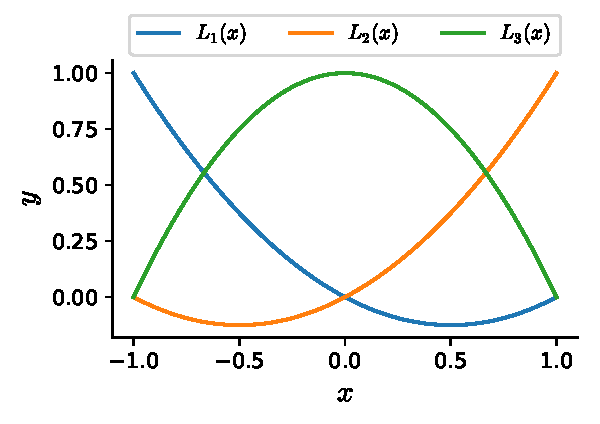
\includegraphics[height=3 in]{interp_base.pdf}
  \caption{Polinomios interpolantes de Lagrange correspondientes a los puntos $x_1 =  -1.0$, $x_2 = 1.0$ y $x_3 = 0.0$}
  \label{fig:interp_base}
\end{figure}

La función o polinomio de interpolación resultante tras realizar la combinación lineal de estos polinomios de acuerdo con
\[p(x) = L_1(x) f_1 + L_2(x) f_2 + L_3(x) f_3\, ,\]
es
\begin{align*}
p(x) &= 10 x^2 + \frac{7}{2}(1 - x)x - \frac{5}{2}(1 + x)x - 10\, .\\
     &= 4x^2 + x - 10
\end{align*}

La función resultante $p(x)$, se compara con la función original $f(x)$ en la \cref{fig:interp_comparacion}. Podemos ver que $p(x)$ (polinomio de orden 2) y $f(x)$ (polinomio de orden 3) no son iguales a largo del dominio. Sin embargo, estas funciones coinciden en los puntos donde $f(x)$ se conocía originalmente.

\begin{figure}[H]
  \centering
  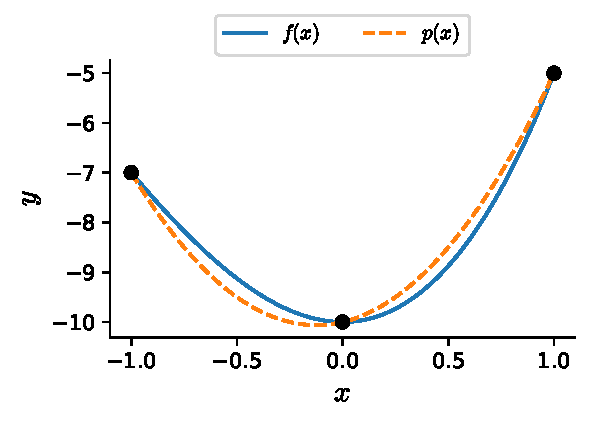
\includegraphics[height = 3 in]{interp_comparacion.pdf}
  \caption{Función de interpolación (en línea punteada) resultante tras aplicar 
  la superposición de la \cref{eq:interp_coef} conjuntamente con los datos de 
  la \cref{tab:interp_tres} (puntos negros) y correspondientes a la función 
  $f(x) = {x^3} + 4{x^2} - 10$ (línea continua) ${x_1} =  - 1.0$, ${x_2} =  
  1.0$ y ${x_3} = 0.0$}
  \label{fig:interp_comparacion}
\end{figure}

Supongamos que además se desea calcular una aproximación a la primera derivada de la función. Para calcular dichas aproximaciones derivamos la \cref{eq:interp_coef} para obtener
\begin{equation}
  \dv{p(x)}{x} = \dv{L_1(x)}{x} f_1 + \dv{L_2(x)}{x} f_2 + \dv{L_3(x)}{x} 
  f_3
  \label{eq:interp_deriv}
\end{equation}

La aproximación resulta ser una combinación lineal de productos entre polinomios interpolantes (que en este caso resultan ser derivadas de los polinomios de Lagrange) y valores conocidos de la función. La derivada obtenida de esta manera se compara con la derivada exacta en la \cref{fig:interp_deriv}.

\begin{figure}[H]
  \centering
  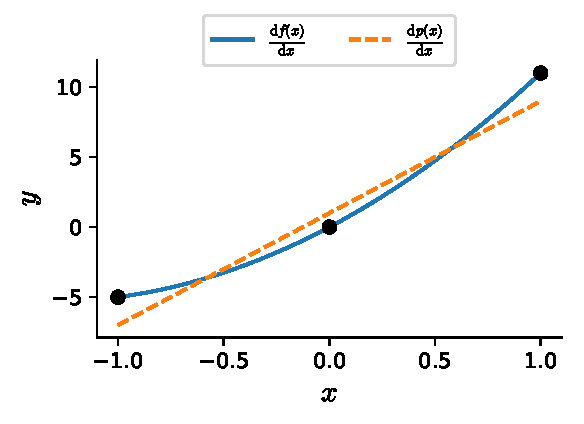
\includegraphics[height = 3 in]{interp_deriv.pdf}
  \caption{Comparación entre la derivada exacta de $f(x)$ y la derivada obtenida a partir de la aproximación con polinomios de Lagrange usando la \cref{eq:interp_deriv}.}
  \label{fig:interp_deriv}
\end{figure}

Se puede observar como ahora la aproximación a la derivada, aunque se acerca a 
los valores reales obtenidos analíticamente, no coincide con estos últimos. 
Esta pérdida de precisión se debe a que en la superposición dada por la 
\cref{eq:interp_deriv} se usan los valores conocidos de $f$ y no los de 
$\dv{f(x)}{x}$ y se usan como polinomios $\dv{L_i(x)}{x}$, los cuales no 
satisfacen la propiedad de interpolación, es decir
\[\dv{L_i(x_j)}{x} \neq \begin{cases}
1,\quad \text{si } i = j\, ,\\
0,\quad \text{si } i \neq j\, .
\end{cases}\]

Con el propósito de asimilar la variación de la solución con los diferentes 
esquemas de interpolación, la \cref{fig:interp_multiple} compara la  
interpolación obtenida por medio de polinomios de orden 1, 2 y 4 para la 
función $f(x) = 2e^{x} + \sin(3x)$. La columna izquierda muestra los polinomios 
interpolantes y la columna derecha los polinomios base $L_i (x)$.

\begin{tcolorbox}
Si usamos interpolación para se aproximar la función de desplazamientos 
entonces también es posible determinar la aproximación a la función de 
deformaciones. Sin embargo, esta última sería una función de más bajo nivel de 
aproximación.
\end{tcolorbox}

\begin{figure}[H]
\centering
  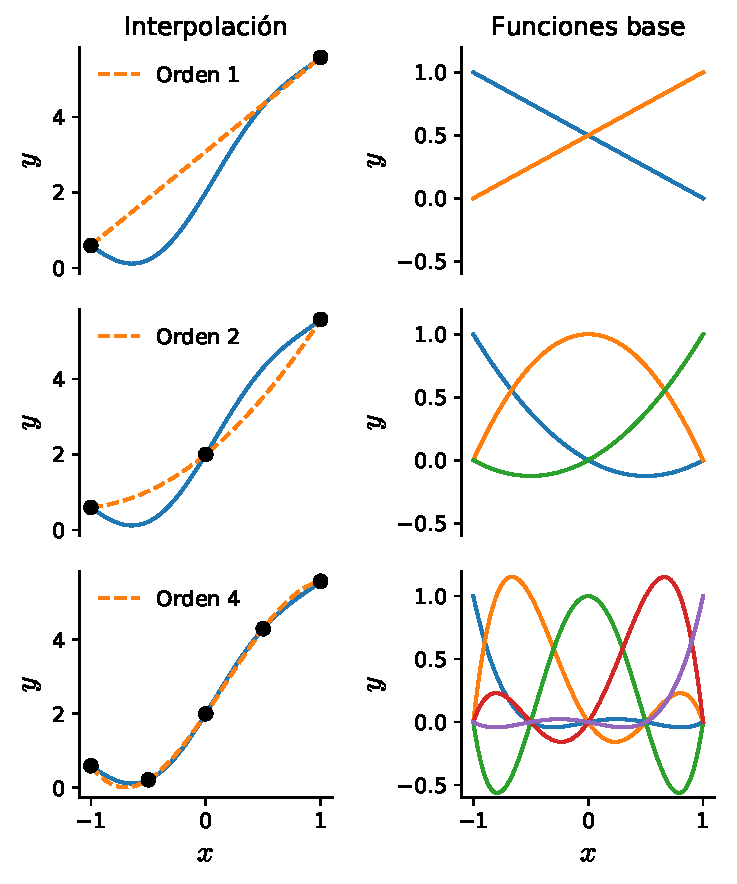
\includegraphics[width=4.5 in]{interp_multiple.pdf}
  \caption{Interpolación para la función $f(x) = 2e^{x} + \sin(3x)$ mediante polinomios de diferente orden.}
\label{fig:interp_multiple}
\end{figure}

Finalmente, la \cref{fig:interp_multiple_deriv} muestra las primeras derivadas de los polinomios de interpolación de orden 4 así como la aproximación a la primera derivada usando la expresión

\[\dv{p(x)}{x} = \sum_{i} \dv{L_I(x)}{x} f_i \, .\]

\begin{figure}[H]
  \centering
  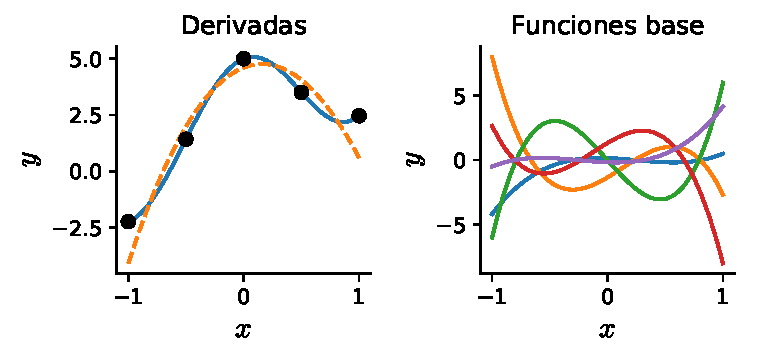
\includegraphics[width=5 in]{interp_multiple_deriv.pdf}
  \caption{Derivadads de los polinomios de interpolación de orden 4 y aproximación a la primera derivada de la función $f(x) = 2e^{x} + \sin(3x)$.}
\label{fig:interp_multiple_deriv}
\end{figure}

\subsection{Distribución de los puntos de muestreo}
Considere la función
\[f(x) = \frac{1}{1 + 25 x^2}\, ,\]
mostrada en la \cref{fig:runge_fun} y en la cual los 11 puntos negros corresponden a nodos o puntos de muestreo donde esta se supone conocida.
\begin{figure}[h]
\centering
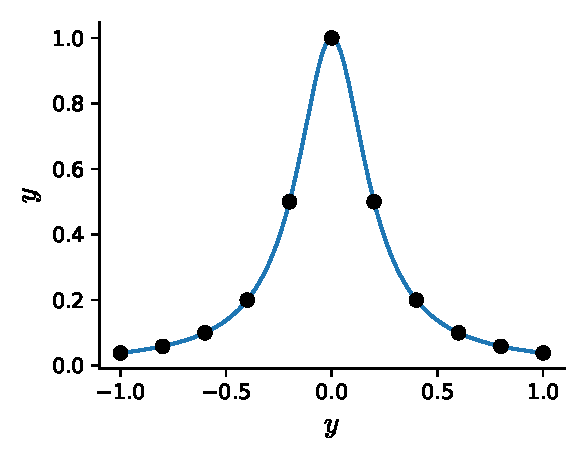
\includegraphics[width=4 in]{runge_fun.pdf}
\caption{Función de Runge $f(x) = \frac{1}{1 + 25{x^2}}$.}
\label{fig:runge_fun}
\end{figure}

Los puntos están separados por una distancia constante $\Delta x = 0.2$. Se desea aproximar la función mediante polinomios de Lagrange usando los 11 puntos de muestreo.

La \cref{fig:runge_equi} muestra los 11 polinomios de Lagrange de orden 10 asociados con los nodos del dominio así como el polinomio de interpolación resultante para aproximar la función. La aproximación es imprecisa en los extremos del intervalo donde se presentan unas fuertes oscilaciones debidas a la distribución equidistante de los nudos.
\begin{figure}[H]
  \centering
  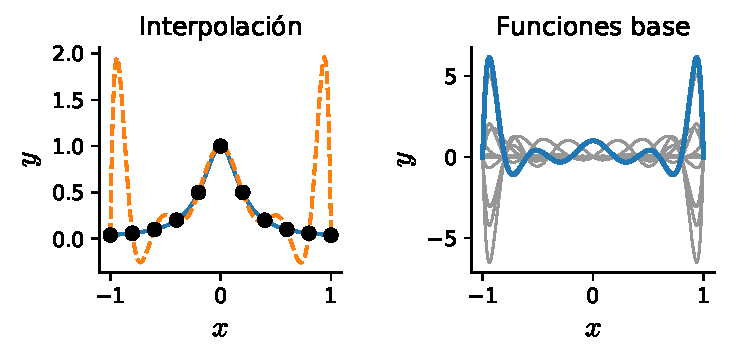
\includegraphics[width=5 in]{runge_equi.pdf}
\caption{Función de interpolación para aproximar la función de Runge usando los puntos de muestreo mostrados en \cref{fig:runge_fun}. A la derecha se muestran las funciones base para esta interpolación, se resalta la función de interpolación para el nodo de la mitad.}
\label{fig:runge_equi}
\end{figure}


La aproximación se puede mejorar variando el espaciamiento de los puntos de muestreo como se muestra en la \cref{fig:runge_cheb} donde los nodos tienen una mayor densidad en los extremos del dominio de solución.

\begin{figure}[H]
  \centering
  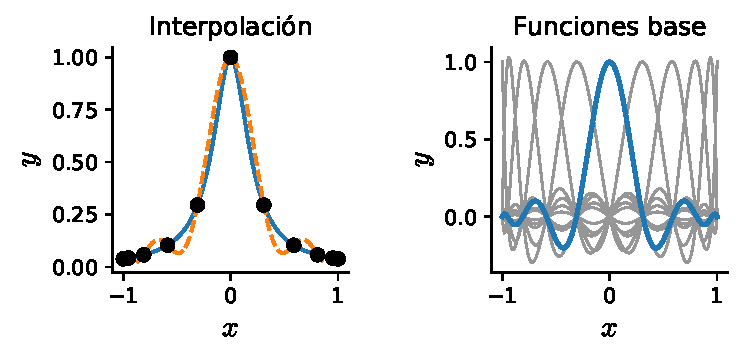
\includegraphics[width=5 in]{runge_cheb.pdf}
  \caption{Función de interpolación para aproximar la función de Runge usando los puntos de muestreo no equidistantes. A la derecha se muestran las funciones base para esta interpolación, se resalta la función de interpolación para el nodo de la mitad. Note que las funciones base toman valores mucho más pequeños que en el caso equidistante.}
\label{fig:runge_cheb}
\end{figure}

Para entender esta patología numérica, relacionada con la distribución de los puntos de muestreo, consideremos los polinomios asociados con el punto central y extremo de la distribución equidistante (\cref{fig:runge_equi}) que se muestran en la parte (a) de la \cref{fig:runge_comparacion}. La traza verde corresponde al polinomio asociado con el nudo central, mientras que la traza azul corresponde al asociado con el nudo extremo. Claramente el polinomio del nudo central introduce la fuerte variación concentrada sobre los extremos del intervalo, mientras que el polinomio del nudo extremo presenta una variación relativamente suave. De manera analoga, la parte (b) de la figura muestra los polinomios central (traza verde) y extremo (traza azul) asociados con la distribución variable de nodos usada para la interpolación de mayor precisión. En este caso ambos polinomios corresponden a una función suave sin concentrar la fuerte oscilación sobre el extremo del intervalo.

\begin{figure}[H]
  \centering
  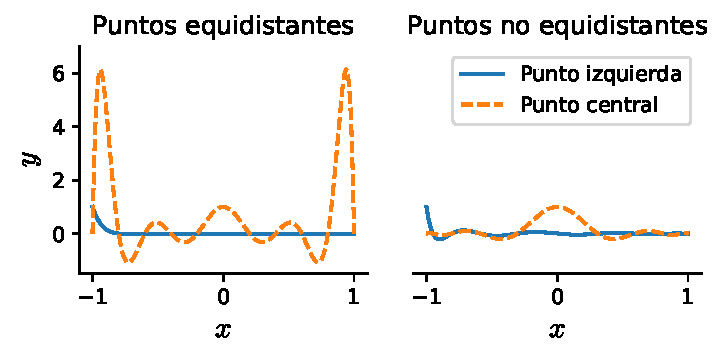
\includegraphics[width=5 in]{runge_comparacion.pdf}
  \caption{Polinomios de Lagrange de orden 10 asociados con el punto inicial y el punto medio para diferentes muestreos.}
  \label{fig:runge_comparacion}
\end{figure}


\subsection{Interpolación local usando una función a tramos}
Como alternativa a la estrategia de usar todos los puntos de muestreo  para realizar la interpolación, también existe la posibilidad de subdividir el intervalo de solución $[x_1, x_n]$, en sub-dominios y realizar la interpolación localmente en cada uno de estos. Por ejemplo la \cref{tab:subdominio} muestra la partición del intervalo $[-1.0, 1.0]$ en sub-dominios conformados por pares de puntos de muestreo consecutivos. En la misma tabla también se muestran los valores de la función $f(x) = {x^3} + 4{x^2} - 10$ en cada uno de los extremos de estos sub-intervalos.

En este caso particular cada subdominio está conformado por un par de puntos y la interpolación se reduce a la determinación de la recta (polinomio de orden 1) que pasa por dichos puntos. Otras alternativas de sub-dominio son posibles, por ejemplo definidos por tres puntos permitiendo una interpolación local de orden 2.
\begin{center}
\begin{tabular}{ccc}
  \hline
  Subdominio & Intervalo & Valores de $f(x)$ \\
  \hline 
   1  & $[-1.0, -0.5]$ & $[-7.000, -9.125]$  \\
   2  & $[-0.5,  0.00]$ & $[-9.125, -10.00]$  \\
   3  & $[+0.0,  +0.5]$ & $[-10.00, -8.875]$   \\
   4  & $[+0.5, +1.0]$ & $[-8.875, -5.000]$   \\
  \hline
\end{tabular}
\captionof{table}{División del intervalo $[-1.0, 1.0]$ en sub-intervalos o subdominios}
\label{tab:subdominio}
\end{center}

La estrategia de interpolación local o por tramos implica el uso de un único conjunto de polinomios, como se muestra en la \cref{fig:interp_local_bases} para el caso de la interpolación lineal en consideración. Nótese que cada par de polinomios interpolantes de grado 1 se repiten en cada uno de los subintervalos.
\begin{figure}[H]
  \centering
  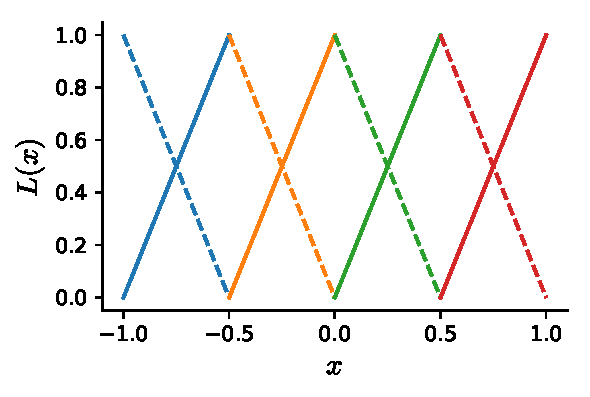
\includegraphics[width=4 in]{interp_local_bases.pdf}
  \caption{Polinomios de interpolación local. Cada dominio tiene dos líneas rectas como base. La interpolación en cada uno de ellos es la combinación lineal estas rectas.}
  \label{fig:interp_local_bases}
\end{figure}


Esta estrategia resulta en una interpolación de la función como la mostrada en la \cref{fig:interp_local_fun} en la cual se aprecia cómo el polinomio de interpolación es ahora una función definida por tramos. Como resultado de la estrategia de interpolación local la primera derivada de la función presenta discontinuidades en los límites de los subdominios, lo cual se aprecia en la parte derecha de esta misma figura. 
\begin{figure}[H]
  \centering
  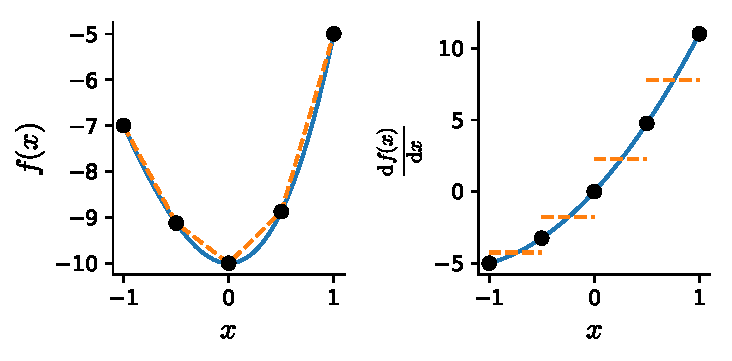
\includegraphics[width=5 in]{interp_local_fun.pdf}
  \caption{Interpolación lineal por tramos de la función $f(x) = {x^3} + 4{x^2} - 10$.}
  \label{fig:interp_local_fun}
\end{figure}

\subsection{Generalización a dominios bi-dimensionales}
Asumamos que estamos interesados en interpolar una función definida en un 
dominio plano (ver \cref{fig:interp_2D}) en el que cada punto se encuentra 
especificado por un vector posición de la forma $\vb{x} = (x, y)$. Por medio 
del problema de interpolación deseamos conocer el valor de la función $f$ para 
un punto $\vb{x}$ suponiendo que conocemos el valor de la función en $n$-puntos 
de la forma $\{(\vb{x}_1, f_1),\cdots,(\vb{x}_n, f_n)\}$. Este problema es la base para resolver el presentado al principio de la sección relativo a la Red Acelerográfica de Medellín.

\begin{figure}[H]
\centering
	\begin{subfigure}[b]{2.5 in}
		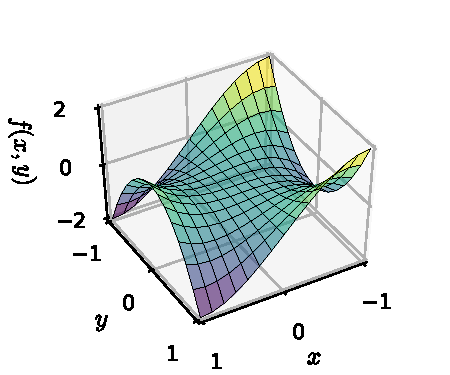
\includegraphics[width=\textwidth]{interp_superficie.pdf}
	\end{subfigure}\,
%
	\begin{subfigure}[b]{2.5 in}
		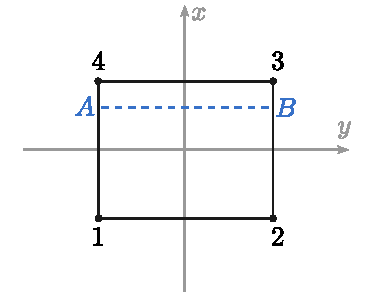
\includegraphics[width=\textwidth]{interp_dominio-2D.pdf}
	\end{subfigure}
\caption{Función $f(x,y)$ sobre un dominio cuadrado con puntos de muestreo rotulados como 1, 2, 3 y 4}
\label{fig:interp_2D}
\end{figure}

Para extender el esquema de interpolación planteado para el caso 1D al actual 
dominio 2D, fijaremos primero $x = x_A$ y realizaremos interpolación 
unidimensional a lo largo de la dirección $y$. Es decir, si consideramos la 
variación de la función en la dirección 1-4, equivalente a $x = x_A$, estaremos 
interesados en saber cual es el valor de la función para un punto arbitrario 
sobre esta línea y con coordenadas $(x_A,y)$ como se ilustra en la 
\cref{fig:interp_1D}.

\begin{figure}[H]
\centering
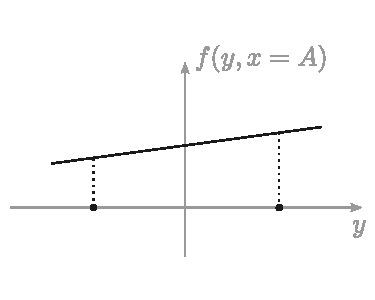
\includegraphics[width=8 cm]{inter1D.pdf}
\caption{Interpolación en la dirección $y$ sobre la línea 1-4.}
\label{fig:interp_1D}
\end{figure}

Usando una expresión análoga a la \cref{eq:interp_pol} se tiene la siguiente solución
\[f(x_A,y) = L_1(y)f_1 + L_4(y)f_4\, .\]
Procediendo de manera similar a lo largo de la línea 2-3 se obtiene
\[f(x_B,y) = L_2(y)f_2 + L_3(y)f_3\, .\]

Ahora nos encontramos en la posición de hacer la interpolación en la dirección 
$x$ usando las aproximaciones $f(x_A,y)$ y $f(x_B,y)$ previamente calculadas, 
escribiendo
\begin{align*}
  f(x,y) &= L_A(x) f(x_A,y) + L_B(x)f(x_B,y)\\
    &= L_A(x)[L_1(y)f_1 + L_4(y)f_4] + L_B(x)[L_2(y)f_2 + L_3(y)f_3]\\
    &= L_A(x)L_1(y)f_1 + L_A(x)L_4(y)f_4 + L_B(x)L_2(y)f_2 + L_B(x)L_3(y)f_3 \, 
    ,
\end{align*}
donde
\begin{align*}
L_A(x) & \equiv L_1(x)\, ,
&L_B(x) & \equiv L_2(x)\, ,\\
L_1(y) & \equiv L_1(y)\, ,
&L_2(y) & \equiv L_1(y)\, ,\\
L_3(y) & \equiv L_2(y)\, ,
& L_4(y) & \equiv L_2(x) \, .
\end{align*}

Los polinomios interpolantes que capturen simultáneamente la contribución en $x$ y en $y$ de cada valor conocido de la función  se forman entonces a partir de productos de polinomios de interpolación unidimensionales dando lugar al siguiente esquema de interpolación
\[f(x,y) = N_1(x,y)f_1 + N_2(x,y)f_2 + N_3(x,y)f_3 + N_4(x,y)f_4\, ,\]
en el cual los polinomios de interpolación $N_i(x,y)$ se definen como

\begin{align*}
N_1(x,y) & = L_1(x)L_1(y)\, ,
&N_2(x,y) & = L_2(x)L_1(y)\, ,\\
N_3(x,y) & = L_2(x)L_2(y)\, ,
&N_4(x,y) & = L_1(x)L_2(y)\, ,
\end{align*}
o, de forma explícita,
\begin{align*}
N_1(x, y) = \frac{1}{4}(1 - x)(1 - y)\, ,\\
N_2(x, y) = \frac{1}{4}(1 + x)(1 - y)\, ,\\
N_3(x, y) = \frac{1}{4}(1 + x)(1 + y)\, ,\\
N_4(x, y) = \frac{1}{4}(1 - x)(1 + y)\, .
\end{align*}


La \cref{fig:interp_4-nodos} muestra los 4 polinomios resultantes que satisfacen la propiedad 
\[N_i (x^j, y^j) = \begin{cases}
1,\quad \text{si } i = j\, ,\\
0,\quad \text{si } i \neq j\, .
\end{cases}\]

\begin{tcolorbox}
En el contexto del método de los elementos finitos para resolver problemas de elasticidad un elemento esta representado por un grupo de nudos, un conjunto de funciones de interpolación del tipo $N_i(x, y)$ correspondientes a cada nudo y estas se usan para aproximar el vector de desplazamientos en cualquier punto del elemento.
\end{tcolorbox}

\begin{figure}[H]
  \centering
  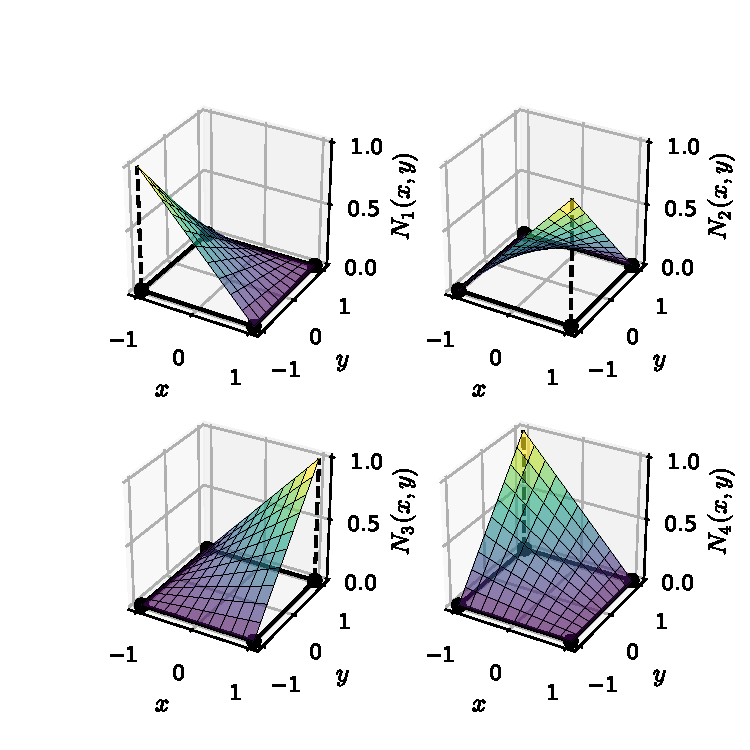
\includegraphics[width=5 in]{interp_4-nodos.pdf}
  \caption{Polinomios de interpolación para un dominio bidimensional con 4 puntos de muestreo.}
  \label{fig:interp_4-nodos}
\end{figure}

\newpage
\subsubsection{Ejercicios}
\begin{enumerate}
	
	\item \label{ejer:inter1} Considere la función $f(x) = x^5 + 4x^3 - 8$ y realice una interpolación de 
	orden 2. Introduzca ahora puntos adicionales de muestreo  para tratar de 
	mejorar la aproximación a la función. Compare los resultados gráficamente 
	mostrando la función exacta, los valores en los puntos de muestreo y el 
	polinomio de aproximación resultante. Realice también la comparación para la 
	primera derivada de la función.
	
	\item \label{ejer:inter2}
	Considere nuevamente la función $f(x) = {x^3} + 4{x^2} - 10$. Genere una tabla análoga a la \cref{tab:subdominio} pero esta vez con al menos 4 sub-dominios cada uno de 3 puntos de muestreo para el intervalo $[-1.0, 1.0]$. Usando lo puntos generados resolver el problema por medio de interpolación local de orden 2. Presentar gráficamente los polinomios interpolantes en los sub-dominios así como la correspondiente función de interpolación. Comparar esta ultima con la definición exacta de la función. Adicionalmente, calcular la primera derivada a partir de la definición exacta de la función y del polinomio de interpolación.
	
\item \label{ejer:inter3}
	Aproximar la función de Runge dada por:
	\[f(x) = \frac{1}{1 + 25x^2}\]
	mediante un esquema local o por tramos usando sub-dominios definidos por pares de puntos. Realizar tramos de longitud constante $\Delta x = 0.2$ y tramos de longitud variable con tamaños menores concentrados en los extremos y aumentando hacia el centro.
	
	
\end{enumerate}
